\chapter{Background}
\section{Turing Machine}
\subsection{Introduction to Turing Machines}
A \emph{Turing Machine} (TM) is a collection $(Q, \Sigma, \delta, q_0)$, where:
\begin{itemize}
    \item $Q$ is a set of states, including the accept state $A$ and reject state $R$;
    \item $\Sigma$ is the set of letters, which does not include the \texttt{blank} symbol;
    \item $\delta \colon Q \setminus \{A, R\} \times \Sigma^+ \to Q \times \Sigma^+ \times \{\texttt{left}, \texttt{right}\}$, where $\Sigma^+ = \Sigma \cup \{\texttt{blank}\}$, is the transition function; and
    \item $q_0 \in Q$ is the starting state.
\end{itemize}
Although based on Turing's work on \cite{turing1936computable}, this definition, along with others in this section, have been adapted from \cite{hopcroft2001automata}.

\begin{figure}[htb]
    \centering
    \begin{subfigure}{0.45\textwidth}
        \centering
        \begin{tikzpicture}
            \node[state, accepting] (q0) at (0, 0) {$q_0$};
            \node[state] (q1) at (2.5, 0) {$q_1$};
            \node[state, fill=green, opacity=0.6] (A) at (5, -1) {$A$};
            \node[state, fill=red, opacity=0.6] (R) at (5, 1) {$R$};
    
            \draw[->] (q0) edge[loop above] node[text width=1.5cm, align=center] {$0 \to 0, R$ $1 \to 1, R$} (q0);
            \draw[->] (q0) -- node[above] {$\# \to \#, L$} (q1);
            \draw[->] (q1) -- node[below, rotate=-20] {$0 \to \#, L$} (A);
            \draw[->] (q1) -- node[above, rotate=20, text width=1.5cm, align=center] {$1 \to 1, L$ $\# \to \#, L$} (R);
        \end{tikzpicture}
        \caption{Full notation}
    \end{subfigure}
    \hfill
    \begin{subfigure}{0.45\textwidth}
        \centering
        \begin{tikzpicture}
            \node[state, accepting] (q0) at (0, 0) {$q_0$};
            \node[state] (q1) at (2.5, 0) {$q_1$};
            \node[state, fill=green, opacity=0.6] (A) at (5, -1) {$A$};
            \node[state, fill=red, opacity=0.6] (R) at (5, 1) {$R$};
    
            \draw[->] (q0) edge[loop above] node {$0|1, R$} (q0);
            \draw[->] (q0) -- node[above] {$\#, L$} (q1);
            \draw[->] (q1) -- node[below, rotate=-20] {$0 \to \#, L$} (A);
            \draw[->] (q1) -- node[above, rotate=20] {$1|\#, L$} (R);
        \end{tikzpicture}
        \caption{Shorthand notation}
    \end{subfigure}
    \caption{A FSM representation of a TM that accepts binary numbers divisible by 2.}
    \label{fig:tm_isDiv2}
\end{figure}

We can represent a TM as a finite state machine (FSM). This is a directed graph, with vertices as states and edges as transitions. An example is given in Figure \ref{fig:tm_isDiv2}. In this case, the alphabet $\Sigma = \{0, 1\}$. The blank symbol is denoted by $\#$. The initial state is denoted by $q_0$; the accept state $A$ and the reject state $R$. Every edge corresponds to an evaluation of the transition function $\delta$, e.g. $\delta(q_1, 0) = (A, \texttt{blank}, \texttt{left})$. 

The figure presents two ways of representing FSM- subfigure (a) shows how all the transitions can be specified, while subfigure (b) only shows the transitions where the tapehead value is getting changed. We will make use of the shorthand FSM representation from now.

\subsection{Executing a TM on a tape}
Let $\Sigma$ be an alphabet. A \emph{tape $T$ on $\Sigma$} is a function $T\colon \mathbb{Z} \to \Sigma^+$. In particular, the tape has infinite entries in both directions. Moreover, $T$ is a \emph{valid tape} if only finitely many symbols on $T$ are not \texttt{blank}, and all the values that can be non-\texttt{blank} are non-\texttt{blank}. That is, there exist integers $a, b$ such that for all $x \in \mathbb{Z}$, $T(x)$ is not \texttt{blank} if and only $x \geq a$ and $x \leq b$. 

We can represent a tape using a figure. For instance, let $\Sigma = \{0, 1\}$, and let $T$ be the tape on $\Sigma$ given below:
\[T(x) = \begin{cases}
    0 & x \in \{0, 2, 3\} \\
    1 & x \in \{1\} \\
    \texttt{blank} & \text{otherwise}.
\end{cases}\]
Then, the following figure represents the tape $T$:
\begin{figure}[H]
    \centering
    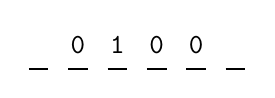
\begin{tikzpicture}
        \draw[thick] (-0.25, 0) -- (0, 0);
        \foreach \x[count=\i] in {0, 1, 0, 0} {
            \draw[thick] (\i*0.5-0.25, 0) -- (\i*0.5, 0);
            \node at (\i*0.5-0.125, 0.3) {\texttt{\x}};
        }
        \draw[thick] (2.25, 0) -- (2.5, 0);
    \end{tikzpicture}
\end{figure}
We will assume that the first non-blank value is at index 0.

A TM can be executed on a tape. Let $M$ be a TM with alphabet $\Sigma$, and let $T$ be a (valid) tape on $\Sigma$. We execute $M$ on $T$ inductively, as follows:
\begin{itemize}
    \item At any point during execution, we maintain 3 objects- a tape on $\Sigma$, a state in $M$ and an index in the tape (called the \emph{tapehead index}). 
    \item At the start, the tape is $T$; the tapehead index is $0$; and the state is the initial state $q_0$. 
    \item At some point during the execution, assume that we have the tape $S$, tapehead index $j$, with \emph{tapehead value} $T(j) = t$, and a non-terminating state $q$ (i.e. not $A$ or $R$). Denote $\delta(q, t) = (q', t', \texttt{dir})$. Then, the next state is $q'$, and the next tape $S'$ and the next tapehead index $j'$ are given by:
    \[S'(x) = \begin{cases}
        t' & x = i \\
        S(x) & \text{otherwise},
    \end{cases} \qquad j' = \begin{cases}
        j+1 & \texttt{dir} = \texttt{right} \\
        j-1 & \texttt{dir} = \texttt{left}.
    \end{cases}\]
    If the state $q'$ is not a terminating state, then the execution continues with these 3 objects. Otherwise, execution is terminated with terminating state $q'$.
\end{itemize}

We illustrate this process with the TM in Figure \ref{fig:tm_isDiv2}. First, a tape on the TM will only have values 0 and 1, and can be thought of as a binary number. So, we can execute the TM on the tape \texttt{100}. In that case, the execution proceeds as follows:
\begin{itemize}
    \item We start at $q_0$ with the tapehead value the first entry, i.e. \texttt{1}.
    \item Since the value is \texttt{1}, we stay at $q_0$ and move the tapehead pointer to the right. Now, the tapehead value is \texttt{0}.
    \item The transition for \texttt{0} and \texttt{1} are the same with respect to $q_0$, so we keep moving to the right until we end up at the blank symbol. At this point, the tape is as follows:
    \begin{figure}[H]
        \centering
        \begin{tikzpicture}
            \draw[thick] (-0.25, 0) -- (0, 0);
            \foreach \x[count=\i] in {1, 0, 0} {
                \draw[thick] (\i*0.5-0.25, 0) -- (\i*0.5, 0);
                \node at (\i*0.5-0.125, 0.3) {\texttt{\x}};
            }
            \draw[thick] (1.75, 0) -- (2, 0);
            \draw[->] (1.875, -0.5) -- (1.875, -0.1);
        \end{tikzpicture}
    \end{figure}
    \item Now, since the tapehead value is \texttt{blank}, we move to the left and the current state becomes $q_1$.
    \item The current value is a \texttt{0}, so we move to the accept state $A$. Hence, the tape gets accepted.
\end{itemize}
As we can see, the state $q_0$ is used to traverse to the first blank symbol (i.e. the end of the string). At that point, we move to the state $q_1$. At this point, we accept the string if and only if the current tapehead value (which is the last entry on the tape) is \texttt{0}. Hence, this TM accepts binary numbers if and only if they are divisible by 2.

\subsection{TM as a model of computation}
TODO

% - Turing Machine as a model of computation
% > Turing established that TMs are the "right" model for computation
% > There are many equivalent models of computation, such as TM, lambda-calculus, (general) recursive functions, etc.
% > Turing showed this by showing that lambda-definable ("effectively calculable", i.e. those a human could do reasonably) functions are Turing computable, and that Turing computable machines are recursive. It was already established that lambda-calculus and recursive functions are equivalent.
% > Lambda-definable functions are a specific type of lambda-terms
% > Thesis since it is somewhat informal- what does right model of computation mean? Used to consider what a human could do.


% TODO: Add some content on \lambda-calculus and Church-Turing Thesis

\section{Parser}
A \emph{compiler} is a program that takes a program in the source programming language (PL) and converts it into a program in some target PL. During the process, the compiler also detects any errors, such as syntax and type errors. 

\begin{figure}[htb]
    \centering
    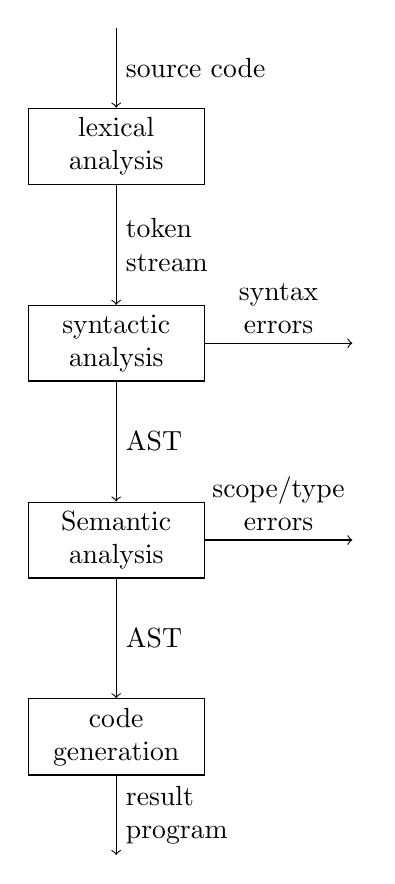
\begin{tikzpicture}
        \node[draw, text width=2cm, align=center] (LA) at (0, 0) {lexical analysis};
        \node[draw, text width=2cm, align=center] (SA) at (0, -2.5) {syntactic analysis};
        \node[draw, text width=2cm, align=center] (CA) at (0, -5) {Semantic analysis};
        \node[draw, text width=2cm, align=center] (CG) at (0, -7.5) {code \\ generation};
        
        \draw[->] (0, 1.5) -- node[right] {source code} (LA);
        \draw[->] (LA) -- node[right, text width=2cm, align=left] {token \\ stream} (SA);
        
        \draw[->] (SA) -- node[above, text width=2cm, align=center] {syntax \\ errors} (3, -2.5);
        \draw[->] (SA) -- node[right] {AST} (CA);
        \draw[->] (CA) -- node[above, text width=2cm, align=center] {scope/type \\ errors} (3, -5);
        
        \draw[->] (CA) -- node[right] {AST} (CG);
        \draw[->] (CG) -- node[text width=2cm, align=left, right] {result \\ program} (0, -9);
    \end{tikzpicture}
    \caption{The data flow between the compilation phases.}
    \label{fig:compilation_process}
\end{figure}

We will now consider the different phases of the compilation process. This is summarised in Figure \ref{fig:compilation_process}. This figure, along with most of the content in this section, has been adapted from \cite{aho2007compilers}.

\subsection{Lexical Analysis}    
First, we perform \emph{lexical analysis} using a \emph{lexer}. 

In this stage, the source code is enriched to make it ready for parsing. In particular, we generate a stream of source code, which reads the program word by word. Then, it produces \emph{tokens}, which are a sequence of words in source code along with labels. For instance, consider the mathematical expression \texttt{1 + 2}. We can convert this expression into 3 tokens: \texttt{(1, NUM)}, \texttt{(+, PLUS)} and \texttt{(2, NUM)}. 

\subsection{Syntactic Analysis}
Next, we try to parse the token stream into an (abstract) syntax tree (AST). If there are syntax errors present in the program, then it is not possible to construct a syntax tree. This will be detected during this phase, at which point we can throw a syntax error.

A syntax tree represents the program as a tree of nodes. Typically, the internal nodes represent operations and the leaves represent their arguments. An AST is a compact representation of a syntax tree that does not feature all the nodes. The abstract syntax tree for the expression \texttt{(1 + 2) * (3 + 4)} is given in Figure \ref{fig:AST_example}.

\begin{figure}[htb]
    \centering
    \begin{tikzpicture}[
        level 1/.style={sibling distance=4cm},
        level 2/.style={sibling distance=2cm},
    ]
        \node[ellipse, draw] {TIMES}
        child {
            node[ellipse, draw] {PLUS}
            child {
                node[draw] {\texttt{1}}
            }
            child {
                node[draw] {\texttt{2}}
            }
        }
        child {
            node[ellipse, draw] {PLUS}
            child {
                node[draw] {\texttt{3}}
            }
            child {
                node[draw] {\texttt{4}}
            }
        };
    \end{tikzpicture}
    \caption{The AST for the expression \texttt{(1 + 2) * (3 + 4)}}
    \label{fig:AST_example}
\end{figure}

There are many ways to parse the stream of tokens. A common method is \emph{recursive-descent} parsing. Here, we recursively parse the source code and generate nodes within the AST. For instance, we initially start by parsing a program. If we then encounter an expression, and this is allowed in the grammar of the language, we parse an expression.

The simplest form of recursive-descent parsing is called \emph{predictive parsing}. This applies when the next token determines what structure it is to be parsed, e.g. if we see the token \texttt{if}, then we know we are parsing an if command. Such a parser makes use of the \texttt{match} method that is used to match the next token value.

A snippet of a recursive-descent class \texttt{CodeParser} is given below, which illustrates how an if statement might be parsed.
\begin{lstlisting}[language=TypeScript]
class CodeParser {
    parseIf():IfContext {
        match("if");
        var condition = parseExpr();
        
        match("then");
        var expr1 = parseExpr();
        
        match("else");
        var expr2 = parseExpr();

        return new IfContext(condition, expr1, expr2);
    }

    // ... other parsing methods
}
\end{lstlisting}

\subsection{Semantic Analysis}
Now, we traverse the AST and check that there were no errors in the source code. Typically, there are 2 types of things to check in this stage- type and scope errors. 

In type errors, we check whether the AST has some type mismatch, e.g. \texttt{1 + true}. If there are no errors, then we will have assigned types to each variable. This information will likely be used during code generation.

In scope errors, we check whether some identifier present in code is undefined. To do so, we need to keep track of all the variables that are in scope at this point. In terms of functions, there is a design choice here- we can have all functions in scope from the start, or add them to scope as they are encountered. 

There are many ways to traverse the AST. One way of doing so makes use of the visitor design pattern (\cite{gamma1995design}). Here, every node in the AST is represent by some child class of the \texttt{Context} class, e.g. \texttt{IfContext} for if statements. The \texttt{Context} class has an abstract method \texttt{accept} that allows us to visit different nodes. We can then make use of this when traversing the AST.

We illustrate the visitor design pattern with an example. So, assume that we have the following class to represent if statements.
\begin{lstlisting}[language=TypeScript]
class IfContext extends Context {    
    accept<T>(validator:CodeVisitor<T>):T? {
        return validator.visitIf(this);
    }

    // ... relevant methods for if context
}
\end{lstlisting}
    In that case, we can define the following method to `visit' an if statement and validate it.
\begin{lstlisting}[language=TypeScript]
class TypeValidator implements CodeVisitor<Type> {
    visit(context:Context):Type? {
        return context.accept(this);
    }
    
    // validate that the condition is of type bool 
    visitIf(ifContext:IfContext):Type? {
        var type = visit(ifContext.condition);
        if (type != Type.BOOL) {
            throw new TypeError("Expected if condition to be of type bool.");
        }
        
        return undefined;
    }

    // ... other validator methods
}
\end{lstlisting}
To run the \texttt{TypeValidator}, we visit the entire program.

The advantage of using the visitor design pattern is that we can traverse all the nodes without altering any of the \texttt{Context} classes; we can just construct another \texttt{Visitor} class. However, if we wanted to add another \texttt{Context} subclass, then we would need to amend all the \texttt{Visitor} classes. We expect the language to be pretty static, so this is perfectly fine in our case.

\subsection{Code Generation}
Finally, we convert the AST into code in the target language. In particular, we traverse the tree left-to-right and convert each phrase from the source language to the target. This can also be done using the visitor design pattern. Here, the return type is expected to be a representation of the target language.
